% Fig. 6 -- Multiplicative gate G(s) (single column, 3.5 in).
% Compile with pdfLaTeX (Overleaf default). Output: fig06_gate_function.pdf
\documentclass[border=3pt]{standalone}
\usepackage[T1]{fontenc}
\usepackage{newtxtext,newtxmath}
\usepackage{tikz}
\usepackage{pgfplots}
\pgfplotsset{compat=1.17}

\definecolor{acc}{RGB}{31,78,121}

\begin{document}
\footnotesize
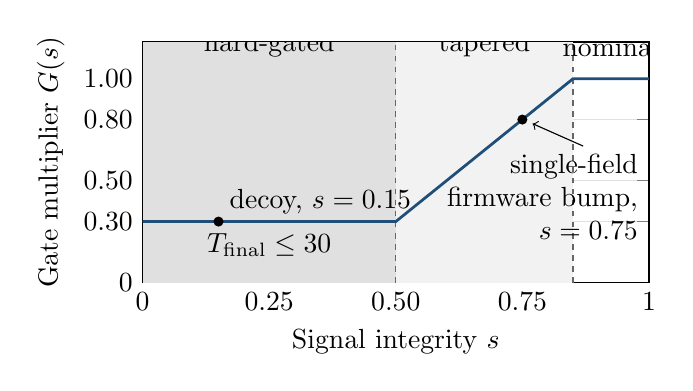
\begin{tikzpicture}
\begin{axis}[
    width=228pt, height=132pt,
    xlabel={Signal integrity $s$},
    ylabel={Gate multiplier $G(s)$},
    xmin=0, xmax=1, ymin=0, ymax=1.18,
    xtick={0,0.25,0.5,0.75,1},
    xticklabels={0,0.25,0.50,0.75,1},
    ytick={0,0.3,0.5,0.8,1},
    yticklabels={0,0.30,0.50,0.80,1.00},
    axis line style={line width=0.5pt},
    tick style={line width=0.5pt},
    ymajorgrids, grid style={black!12,line width=0.3pt},
    clip=true,
]
  % region shading (back to front)
  \path[fill=black!12] (axis cs:0,0)    rectangle (axis cs:0.5,1.18);
  \path[fill=black!5]  (axis cs:0.5,0)  rectangle (axis cs:0.85,1.18);

  % region boundaries
  \draw[black!60,dash pattern=on 2pt off 2pt,line width=0.4pt] (axis cs:0.5,0)  -- (axis cs:0.5,1.18);
  \draw[black!60,dash pattern=on 2pt off 2pt,line width=0.4pt] (axis cs:0.85,0) -- (axis cs:0.85,1.18);

  % region labels
  \node[anchor=south] at (axis cs:0.25,1.06)  {hard-gated};
  \node[anchor=south] at (axis cs:0.675,1.06) {tapered};
  \node[anchor=south] at (axis cs:0.925,1.06) {nominal};

  % the gate
  \addplot[acc,line width=1.0pt] coordinates {(0,0.3) (0.5,0.3) (0.85,1.0) (1,1.0)};

  % worked points
  \addplot[only marks,mark=*,mark size=1.6pt,black] coordinates {(0.15,0.3) (0.75,0.8)};
  \node[anchor=south west,inner sep=2pt] at (axis cs:0.16,0.31) {decoy, $s=0.15$};
  \node[anchor=north east,inner sep=2pt,align=right] at (axis cs:0.99,0.66) {single-field\\firmware bump,\\$s=0.75$};
  \draw[->,line width=0.4pt] (axis cs:0.87,0.67) -- (axis cs:0.77,0.78);
  \node[anchor=north,inner sep=2pt] at (axis cs:0.25,0.27) {$T_{\mathrm{final}}\le 30$};
\end{axis}
\end{tikzpicture}
\end{document}
